%%%%%%%%%%    PREAMBLE    %%%%%%%%%%
\documentclass{article}
\usepackage{rotating}

\usepackage{tikz}
\usepackage{titletoc}
\usepackage{graphicx}
\usepackage{caption}
\usepackage{url}
%%%%%%%%%%%%%%%%%%%%%%%%%%%%%%%%%%%%

\begin{document}

%%%%%%%%%%    COVER    %%%%%%%%%%
\begin{titlepage}

\begin{tikzpicture}[remember picture,overlay]
    \fill[color=black] (current page.north west) rectangle ++(5cm,-\paperheight);
    \node[anchor=south west, text=white] at (current page.south west) {\hspace{1.5cm}\begin{turn}{90}
    \resizebox{!}{40pt}{\hspace{0.4cm}Software Design Document}\end{turn}};
\end{tikzpicture}

\begin{flushright}

\vspace{7.5cm}

\Huge{Regional Transport Service}

\vspace{0.5cm}

\large{Coastal Lancashire Area}

\vspace{8cm}

\normalsize{January, 2026}

\end{flushright}

\end{titlepage}
\newpage
%%%%%%%%%%%%%%%%%%%%%%%%%%%%%%%%%%%%%%%%%%%%

%%%%%%%%%%    LIST OF CONTENTS    %%%%%%%%%%
\tableofcontents
\newpage
%%%%%%%%%%%%%%%%%%%%%%%%%%%%%%%%%%%

%%%%%%%%%%    CONTENT    %%%%%%%%%%
\section{Project Overview}
This document acts as a proposal for development of a regional transport application, for residents and tourists alike, commissioned by the local authority responsible for the coastal area between Preston and Lancaster, including Blackpool, the Fylde and the Wyre coast. The primary deliverable of this project will be a [@TODO], accompanied with the appropriate documentation and evaluation of testing. The nature of this project is solely a software application where no changes to current infrastructure will be made.
\newpage

\section{Background, Context and Scope}
The local authority has issued A strategic priority in support of economic development, environmental sustainability, and social inclusion across the region. The fragmentation of information provision is A key barrier to greater public transport adoption. \\

\subsection{Problem Context and Need for Integration}
Currently, the region is served by multiple transport operators, each maintaining independent timetables and journey-planning systems. These systems operate largely in isolation, making it difficult for users to plan journeys that involve multiple operators or modes of transport. The resulting complexity disproportionately affects infrequent users, visitors, and residents of rural or poorly connected communities. \\

Although a number of commercial journey-planning applications attempt to aggregate transport information across operators, such solutions often introduce additional limitations. These may include financial costs to operators or users, the presence of intrusive advertising, or incomplete coverage that excludes smaller operators delivering socially necessary services. \\

In response to these challenges, this document sets out the rationale and requirements for an integrated transport application designed to provide comprehensive, reliable, and user-centred journey planning across the region. The proposed system seeks to unify transport data from all relevant operators, support robust and accessible route selection, and contribute to a more coherant and attractive public transport network for residents and visitors alike.

\subsection{Scope}
This section defines the scope of the proposed integrated transport journey planning application. It outlines the functionality, users, and geographic coverage included within the project, as well as specific exclusions and constraints. The scope is intended to provide clear boundaries for the system's development and to ensure a shared understanding of what the project will and will not deliver. \\

\subsubsection{In-scope}
\begin{itemize}
    \item Development of an integrated journey-planning application covering all participating transport operators within the region.
    \item Support for multi-operator and multi-modal journey planning
    \item Provision of near-real-time service information, where avaliable
    \item A user-facing interface designed to be accessible to infrequent visitors 
    \item Route planning based on criteria such as journey time, number of interchanges, walking distance, and service availability
\end{itemize}

\subsubsection{Out-of-scope}
The following items are strictly outside the scope of this project
\begin{itemize}
    \item Ticket purchasing, fare payment, or revenue apportionment between operators
    \item Changes to existing transport services, route, or timetables
    \item Ownership or operation of transport services
    \item Advertising-led or commercial data modification features
    \item Guaranteeing data quality beyond what is supplied by operators
\end{itemize}

\subsubsection{Geographic Boundaries}
The system will cover transport services operating within coastal Lancashire between Preston and Lancaster including Blackpool, The Fylde, and The Wyre coast.

\begin{figure}[htbp]
    \centering
    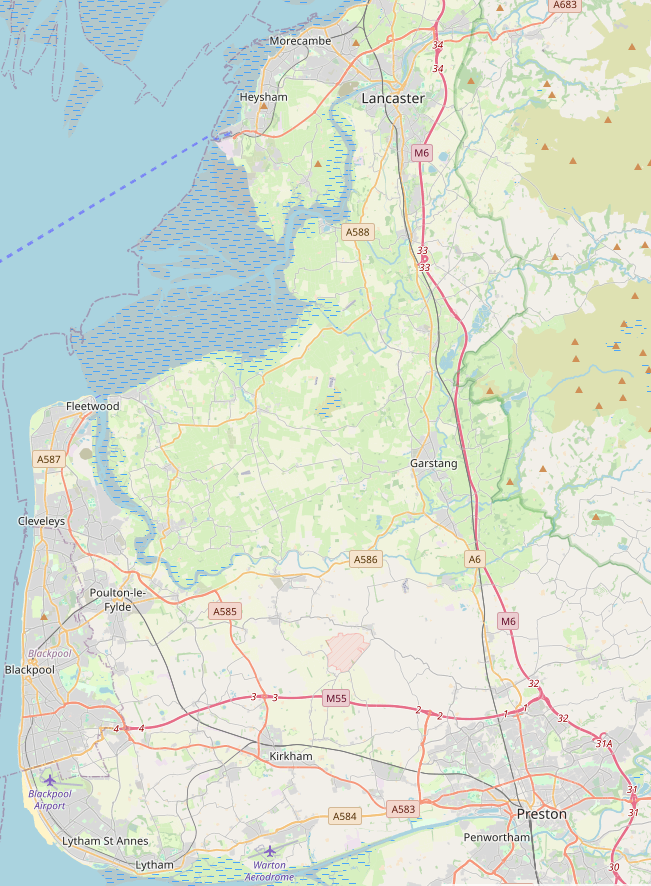
\includegraphics[width=0.5\textwidth]{images/geographical_scope}
    \caption{Map of area covered by scope\cite{OpenStreetMap}}
    \label{fig:app-interface}
\end{figure}

Participation of operators is subject to data availability and cooperation
\newpage

\subsubsection{Target Users}
\begin{itemize}
    \item Residents making regular or occasional journeys
    \item Infrequent users and visitors unfamiliar with the transport network
    \item Users in rural or poorly connected communities
    \item Accessibility needs, including users with reduced mobility or limited digital confidence
\end{itemize}
\newpage

\section{Technological Requirements}
\newpage

\section{Project Milestones}
\newpage

\section{Testing Protocol}
\newpage

\section{Project Budget}
\newpage

\section{Protocol for Acceptance}
\newpage

\bibliographystyle{plain}
\bibliography{references}
%%%%%%%%%%%%%%%%%%%%%%%%%%%%%%%%%

\end{document}
